\chapter{Modelling catchment hydrogeomorphic sensitivity to rainfall radar data resolution}
\chaptermark{Catchment sensitivity to rainfall resolution}

\begin{abstract}
Landscapes evolve and take their shape from the cumulative effect of `geomorphically effective' events. In temperate climates, these are rainfall-driven events of sufficient magnitude to trigger threshold-dependent erosional processes. This chapter investigates the sensitivity of two end-member erosional models to the spatial resolution of rainfall input to a catchment using three historic severe rainfall events in Northern England and Cornwall.

It is demonstrated that the erosional model chosen exerts first-order control of the total amount of landscape change and sediment flux. However, both end member models show sensitivity to the spatial resolution of rainfall input data during individual, formative rainfall events. 

\end{abstract}
\section{Introduction}

Landscape evolution at the catchment scale is punctuated by intense erosive episodes driven by flood events (Wolman and Miller, 1960; Newson, 1980; Costa and O'Connor, 1995) interspersed with periods of relative calm and little geomorphic change, an idea that harks back to the early ideas of geological `catastrophism' (Cuvier, ?). It is these erosive events, driven by intense rainfall in temperate climates, separated by long periods of stasis, that cumulatively sculpt the landscape over geological time. The importance of these rare but formative events has been revisited by recent work such as Huang and Niemann (2006), looking at the long term implications of different geomorphically effective event discharges on fluvial incision; Gupta et al., (2007); Lamb and Fonstad (2010); and Baynes et al., (2015) where the amount of bedrock erosion during a single large flood event was quantified. Still, our understanding of catchment scale landscape evolution is far from complete - the role of individual events is highly variable. Anton (2014) report that rapid gorge formation can be driven primarily by small to moderate sized floods, rather than floods of extreme magnitude. Further, there was no observed relationship between flood magnitude and erosion rate. Turowski et al. (2011) report that streams within catchments can exhibit different behaviour in response to the same flood event -- some streams may erode during high flows, whereas others may deposit during high flows. During small--medium flows their respective behaviour is reversed. Wong et al. (2015) establish through numerical modelling that geomorphic changes in channel geometry during severe flood events are substantial enough to change hydrological response of a river catchment. Catchment-scale erosional dynamics are complex, and except in the simplest cases depend on other forcings other than the magnitude alone of single flood events.  The understanding of hydrogeomorphic processes during single storm events is not only important for the long-term evolution of landscapes, but also for prediction of how catchments will respond to changing hydro-meteorological conditions that may accompany climate change (Kendon et al., 2014).

The focus in this paper is to quantify the sensitivity of catchment-scale erosional processes to the spatial distribution of rainfall during flood events. The assumption of uniform rainfall over a river catchment is argued to hold true for small catchments (Solyom and Tucker 2004; Tucker 2010), but even over small areas, mesoscale rainfall features, such as localized convective storm cells, can result in spatially and temporally uneven input of precipitation into the catchment. In the case of intense convective precipitation, individual storm cells can be as small as 10km$^2$ in areal extent (Weisman and Klemp, 1986; Von Hardenberg et al., 2003). Over larger catchments, or those with steep topographic gradients, precipitation is almost certain to vary spatially, due to orographic enhancement of rainfall (Roe, 2005). As such, rainfall-runoff generation, local river flow, and erosion rates may vary considerably within individual drainage basins. 

Patterns of rainfall distribution across a catchment can affect hydrograph response, including the peak discharge and local water levels (Nicotina et al., 2008). As many geomorphic processes are threshold dependent (Schumm, 1979), such as fluvial incision into bedrock (Sklar and Dietrich, 2001; Snyder et al., 2003), there is potential for the spatial distribution of rainfall to control local erosion rates within a catchment. Non-linearity in geomorphic process laws (e.g. Coulthard et al., 1998; Phillips, 2003; Coulthard and Van de Wiel, 2007) should dictate that catchments are also geomorphically sensitive to the spatial distribution of rainfall. 

Numerical models of landscape evolution usually omit a realistic distribution of rainfall input in favour of uniform, homogenised precipitation across the landscape. When precipitation is `lumped', either spatially or temporally in a catchment, local minima and maxima of precipitation are lost, and with discharge being a function of rainfall rate, this uncertainty propagates through to local discharges and erosion rates. The uncertainty in erosion rates is potentially exacerbated by the non-linearity and threshold dependence of erosive processes. The variability of precipitation is considered in many cases to be as important as total precipitation amount in determining erosional effectiveness (Tucker and Bras, 2000; Tucker, 2010). What is currently lacking in landscape evolution studies is a fuller understanding of how landscapes erode during individual storms, and in particular how erosional processes are sensitive to the details of precipitation across a catchment. 

In numerical models of landscape evolution, resolving the precise temporal and spatial details of rain storms and the hydrological response is often computationally prohibitive, especially over long timescales, and as such modellers have taken to using simpler parametrisiations of storm characteristics, such as using simple stochastic models to generate rainfall inputs and rainfall timeseries (Eagleson, 1978; Tucker et al., 2001). In studies of long term landscape evolution, the sensitivity of landscapes to the spatial distribution of rainfall has been investigated to some extent -- particularly the imprint of orographic precipitation on landscapes (e.g. Roe 2002; Anders 2008; Han and Gasparini, 2015). 

Rainfall resolution has been demonstrated to exert a control over sediment yields over seasonal and decadal timescales (Coulthard and Skinner, 2016). In a numerical modelling study of the River Swale catchment, Coulthard and Skinner show that local as well as catchment-wide sediment yields were predicted to increase by orders of magnitude as rainfall data resolution increases. The study looked at the effects of rainfall spatial data resolution as well the temporal resolution of data, showing both to demonstrate a control over sediment fluxes in a catchment. 

%The intermediate stage between rainfall episode and geomorphic process is the hydrological response of the landscape. This is determined by a range of factors, includng antecedent conditions, bedrock and soil properties, vegetative cover, catchment morphology and the distribution of the rainfall across the catchment. Again, in numerical models of long term landscape evolution, these processes are parameterised for computational efficiency, generally through the selection of an appropriate rainfall-runoff model for the catchment (Beven). Most models of longer term landscape evolution assume a hydrological steady-state during each erosive event, and erosion is calculated as a function of peak or total discharge during a storm. Notable exceptions include the work of Solyom and Tucker (2004), where a parameterised non-steady state rainfall-runoff model is proposed to explain landscape evolution under condtions of short storm duration realtive to runoff time. 
%Talk about some of the purely hydrologic studies that have used spatially varible dsitributed rainfall.

In contrast to previous studies, this paper looks at the effects of individual severe rainfall events using a range of erosional end-member models. The study investigates the sensitivity of catchment-scale erosion to the spatial details of severe rain storms -- the agents of long term landscape evolution. Landscape response is investigated using a numerical landscape evolution model that incorporates a dynamic (non steady-state) water-routing component and a range of fluvial incision and sediment transport laws. A series of model experiments is presented to test how sensitive real landscapes are to the catchment-scale details of precipitation during intense rainfall events. The simulations are each based on selected severe storms in Great Britain occurring in the past decade, which left significant flooding, damage, and geomorphic change in their wake.

The following questions are explored through the use of numerical modelling simulations;

\begin{itemize}
\item Are fluvial erosion and sediment transport processes sensitive to the details of precipitation at the catchment scale during single storm events?
\item Does the choice of erosional model operating within the catchment influence sensitivity to rainfall patterns? 
%\item What is the link between the spatial pattern of rainfall and spatial pattern of erosion and deposition in each storm--flood event?
\item What are the implications of this for longer term landscape evolution? 
\end{itemize}

%%%%%%%%%%%%%%%%
\section{Theory}
%%%%%%%%%%%%%%%%
In our conceptual model of landscape evolution, fluvial processes -- erosion and deposition of sediment and bedrock by flowing water -- are assumed to be the dominant geomorphic processes at work. The numerical model used to simulate these processes uses established hydrological and geomorphic process laws, which are breifly reviewed here in the following sections.

\subsection{Rainfall-runoff and flow routing}
From rainfall input, runoff is calculated using an adaptation of the Beven and Kirby (1979) TOPMODEL. Total surface and subsurface discharge is given by:

\begin{equation}
Q_{tot} = \frac{m}{T}\log \left( \frac{(r - j_t) + j_t \exp \left( \frac{rT}{m} \right) }{r} \right)
\end{equation}

where \(T\) is the time step in seconds, \(r\) is the rainfall rate, \(j_t\) is a function that describes soil moisture store, and \(m\) is a parameter that controls the rise and fall of this soil moisture store in \(j_t\). These adapted TOPMODEL equations are given fully in Coulthard (2002), equations (1) and (2).

The amount of water partitioned between surface and subsurface flow is determined by a simple infiltration threshold, given by:

\begin{equation}
I_t = KS(Dx)^2
\end{equation}

where \(K\) is hydraulic conductivity, \(S\) is the slope, and \(Dx\) is the width of the grid cell or horizontal grid spacing. The infiltration threshold is subtracted from \(Q_{tot}\) to give the portion of water routed over the surface.

Surface water and channel flow is an important driver in catchment scale erosional processes. The amount and velocity of water flow is a variable in both the sediment transport and bedrock erosion laws. The water flow equations are based on a simplified form of the shallow water flow equations, a simplification first derived by Bates (2010) and incorporated into the landscape evolution model by Coulthard et al (2013). The flow between cells is calculated by:

\begin{equation}
Q = \frac{q - g h_{flow} \Delta T \frac{\Delta (h+z) }{\Delta x}}{1 + g h_{flow} \Delta t n^2 |q| / h_{flow}^{10/3}} \Delta x
\end{equation}

where \(q\) is the water flux between cells from the previous iteration, \(g\) is acceleration due to gravity, \(h_{flow}\) is the maximum depth of flow between cells (m), \(t\) is time (s), \(h\) is depth of water, \(z\) is elevation, \(x\) is the grid well width, and \(n\) is Manning's roughness coefficient. The full implementation details are given in Coulthard (2013), and the derivation from the shallow water equations is given in Bates (2010).

\subsection{Sediment transport}
Transport of loose sediment within the model is governed by the \citet{Wilcock2003} sediment transport model. The Wilcock and Crowe model represents transport of mixed sand/gravel fractions based on the surface sediment composition. The rate of sediment transport, \(q_i\), is given as:

\begin{equation}
q_i = \frac{F_i {U_*}^3 {W_i}^*}{(s -1) g}
\end{equation}

where \(F_i\) is the fractional volume of sediment, for a given sediment fraction, \(i\), \(U^*\) is the shear velocity, \(s\) is the ratio of sediment to water density. \({W_i}^*\) is a function relating fractional transport rate to total transport rate (see \citet{Wilcock2003} for a full derivation of this equation). The usage of this sediment transport model is extrapolated here to account for finer particles such as silts \citep{Vandewiel2007}, as well as the sand-gravel mixture it was originally designed for.

\subsection{Bedrock incision}
\label{bedrock_model}
A simple model of bedrock incision based on the excess shear stress model (Citations) is implemented in the numerical model. The rate of bedrock incision is determined by the amount of shear stress acting on the bedrock, above a threshold level of stress required to initiate substrate removal (e.g. \citet{Snyder2003}. When bedrock material is removed, it is distributed amongst the sediment fractions according to the fractional proportions set by the user. The rate of bedrock erosion according to the excess shear stress model is given by:

\begin{equation}
\varepsilon = k_e(\tau_b - \tau_c)^{P_b}
\end{equation}

where \(k_e\) is the bedrock erodibility coefficient, \(\tau_b\) is the basal shear stress on the channel bed, \(\tau_c\), is the critical shear stress threshold, \(P_b\) is the shear stress exponent. (Cite Howard or Whipple?)

%%%%%%%%%%%%%%%%%%%%%%%%%%%%%
\section{Experimental design and case study descriptions}
%%%%%%%%%%%%%%%%%%%%%%%%%%%%%
Three upland catchments in the UK were selected to represent a range of catchment sizes and shapes. The catchments were also chosen on the basis that they had experienced a severe rain storm which could be used as a basis for the experiments, such that it could be considered `extreme' in the typical return period of flooding events for each particular catchment. Peak discharges for each of the following flood events exceed the 99th percentile for their respective catchments. The catchments and respective severe rain events chosen were located in: Ryedale, North Yorkshire, 2005; Eden, Cumbria 2012; and Boscastle, Cornwall, 2004. An overview map of their locations is given in Figure \ref{overview_fig}. A table (Table \ref{met_setting}) summarises the key features of each catchment and associated storm.

\linespread{1.3}
\begin{table}
\resizebox{\textwidth}{!}
{%
\begin{tabular}{l c c c} \hline

Catchment Name& \textbf{Eden} 			& \textbf{Ryedale} &  \textbf{Valency} \\ \hline
Catchment Area & 2286km$^2$ 			& 270km$^2$ 				& 18km$^2$ \\ 
Catchment Type & Upland-Lowland & Upland, Moor/Peaty & Upland, Pasture \\ 
Storm Date	 		&  2005-01-07	 & 2005-06-19 	& 2004-08-16 \\ 
Peak Rainfall	 (mm hr \(^{-1}\)) & & 125  & c.400 \\
Peak Discharge	 	& & & \\ 
Meteorological Setting	& 	& Split-front, convective system & Quasi-stationary convective system \\ 
3hr Rainfall Return Period 		& (tbc)	 & 330yr (Wass et al. 2008)	& 1300yr (Burt, 2005) \\ \hline
\end{tabular}
}
\caption{Table showing key characteristics of each storm event.}
\label{met_setting}
\end{table}

\subsection{Meteorological setting}

\subsubsection{Boscastle, Cornwall storm 2004}
The Boscastle storm took place on the 16th August 2004 leading to flooding within the River Valency catchment and the village of Boscastle. The extreme rainfall accumulations of up to 200 mm in the upper Valency catchment resulted from prolonged rainfall between the hours of 1200 -- 1600 UTC. Rainfall rates were thought to have reached almost 400 mm hr\(^{-1}\) \citep{Golding2006}, after correcting for under-reporting from rain gauges in the vicinity of the catchment. (Burt, 2006).

The meteorological conditions that enabled such prolonged heavy rainfall were a combination of large-scale synoptic conditions moving in from the Atlantic, with moist lower atmospheric layers readily forming convective cloud. Repeated initiation of convection along the north Cornish coast lead to what appeared to be relative stationary convective cells over the Valency catchment. Later authors refer to this type of convective storm as a 'Boscastle-type' or quasi-stationary convective storm (cite the reading person).

\subsubsection{Ryedale, North York Moors storm 2005}
The Ryedale storm occurred on 19 June 2005. Intense rainfall throughout the afternoon lead to total accumulated rainfall amounts of up to 89mm in the Ryedale valley, between the hours of 1400 -- 1800 UTC. Peak instantaneous rainfall rates were estimated to have been around 32.5mm hr\(^-1\) (Sibley et al., 2009) to 59.4 mm hr \(^{-1}\) (Hopkins et al. 2010), though one report states they reached as high as 125 mm hr \(^{-1}\) (Cinderley, 2005). The antecedent conditions had been dry for a prolonged spell, leading to cracking of the surface peat in the higher elevations of the catchment.

The meteorological conditions leading to such heavy rainfall was a combination of a cold, upper-level air mass advecting over a warm moist boundary layer, leading to unstable conditions that enabled a convective thunderstorm to develop in the late afternoon. The instability was enhanced by a split-frontal system. [More? Too much met here?]. The conditions let to a particularly high amount of precipitable water present in the atmosphere which was subsequently washed out into the landscape during intense rainfall. 

\subsubsection{Eden Valley, Carlisle, 2005}

\subsection{Numerical model set-up}
The landscape evolution model developed in Chapter 3 (Working name: HAIL-CAESAR) is used to carry out numerical simulations based on the three catchments and corresponding storm events. HAIL-CAESAR is a cellular automaton landscape evolution model based on the CAESAR-Lisflood model (Coulthard et al., 2013). The HAIL-CAESAR model simulates a range of fluvial erosion and sediment transport laws. The model also interpolates and downscales rainfall input data to higher resolutions and this feature is used in the group of simulations with the 5m interpolated radar rainfall data. 

\subsubsection{Erosion model choice}
A variety of erosion laws exist describing how landscapes erode from fluvial incision. The choice of erosion law for a given catchment depends on a variety of factors, such as the characteristic substrate material in the catchment -- is it predominantly loose sediment or cohesive, solid bedrock? In reality, landscapes are often a mixture of these two extremes, incorporating loose sediment on top of solid bedrock. Catchments also often exhibit a transition from rockier upland headwaters, to more thickly soil-mantled flood plains. In order to address the uncertainty in choosing which erosion model applies for each catchment (Section \ref{theory}), two erosion model end-members are used, with each one representing a different conceptual model of fluvial incision and sediment transport. These include: i) a purely sediment transport-limited model, ii) a detachment-limited bedrock incision model. The equations describing the transport-limited and detachment-limited models are discussed in Section \ref{theory}. Further models were considered, such as a hybrid transport-detachment limited erosion model, but it was deemed beyond the scope of this study, which is to focus on the sensitivity of rainfall resolution, rather than wide range of erosion and sediment transport models. 

A set of control simulations modelling only runoff and water routing (no erosional model) were also carried out for comparison against the two erosion end-member simulations. In total a series of 9 simulations were carried out -- three for each of the three catchments.

%\paragraph*{Hybrid model}
%The hybrid model assumes a limited-depth sediment layer, overlying a bedrock layer. Figure \ref{hybrid_model} shows a typical cross section through a typical valley in the hybrid model set-up. In the initial model state (before the spin-up period), a channel is 'burnt-in' to the sediment-layer. Whenever bedrock becomes exposed during the hybrid simulation, the simple detachment-limited erosion law is applied. Material removed from the bedrock layer is then apportioned between the various sediment fractions. At all other times, the sediment transport law applies to the sediment layer. 

\subsubsection{Rainfall spatial resolution}
In order to assess the sensitivity of each erosional model to the spatial details of precipitation, three different spatial resolutions of rainfall input are used in each simulation. All three are based on the same original rainfall source data - the UK NIMROD radar data product. Only the spatial distribution and resolution of rainfall is assessed in this study -- other studies have previously investigated the effects of the temporal resolution of rainfall data on discharge and erosion rates (e.g Nicotina et al., 2008; Coulthard and Skinner, 2015; Coulthard, 2013b). Three levels of rainfall detail are used: 

\begin{itemize}
\item Uniform or 'lumped' precipitation -- radar-derived rainfall rates across the catchment are spatially-averaged to produce a basin-wide average rainfall rate.  
\item Gridded rainfall input. The rainfall is input from a overlying gridded mesh of raincells, at the same resolution as the radar product (1km).
\item Interpolated rainfall input. The radar data is interpolated to the same resolution as the topography grid (i.e. 50m). \textit{(Interpolation method TBC - but see study by Tait et al (2006) and perhaps implement their method) }
\end{itemize}

The reason for running a simulation with an interpolated rainfall data set is to reduce the effect of harsh gradients between adjacent cells, as is sometimes apparent when using the rainfall data at its native resolution of 1km. Figure \ref{rainfall_input} gives an indicative illustration of this. A matrix of experiments is shown in Table \ref{model_setting}.

%\subsubsection{Model spin-up}
%
%The HAIL-CAESAR model (Valters ?\& Coulthard?, 2016/7) initialises the model domain with a uniform distribution of sediment grain sizes across the catchment. This is physically unrealistic, so the model domain is `spun-up' for a simulated time of 1000 days using typical rainfall data for each catchment. This ensures a heterogeneous distribution of sediment throughout the catchment prior to the detailed storm simulations. 

\section{Sensitivity analysis}
There are numerous user defined parameters in the HAIL-CAESAR model, and in landscape evolution models in general, that have a wide range of potential values. Parameter selection in environmental modelling comes with a degree of uncertainty, and resulting outputs from models can be highly sensitive to the user's choice of input parameters for a given simulation \citep{Pelletier2012}. Initial testing of the HAIL-CAESAR model, and studies using the CAESAR-Lisflood model that it is based upon show it is particularly sensitive to the TOPMODEL \textit{m} parameter, a parameter that controls the rise and fall of the soil moisture store, and hence how a river catchment responds to rainfall input \citep{Beven1979}. 

To assess the sensitivity of the model to the choice of TOPMODEL-\textit{m} parameter, a series of simulations were carried out with a range of \textit{m} values for both test cases. Simulations of each flood event were carried out with the \textit{m} values shown in table \ref{table-m-sens}.

\begin{table}
\begin{tabular}{lc}
\textbf{Catchment} & \textbf{TOPMODEL \(m\) parameter} \\
\hline
Boscastle  &                                            \\
Ryedale     & 0.03, 0.04, 0.05, 0.06, 0.07, 0.08, 0.09, 0.1, 0.15, 0.2  \\
\hline
\\ 
\end{tabular}
\caption{TOPMODEL \(m\) parameter values used to run sensitivity simulations for each catchment.}
\label{table-m-sens}
\end{table}

%%%%%%%%%%%%%%%%%
\section{Results}
%%%%%%%%%%%%%%%%%
\textit{I intend to discuss the spatial differences in erosion, as well as any differences in basin-wide average erosion rates, and explain these differences by referring back to the Theory section.}

The discussion will be aided by figures showing (for each of the three rainfall input variations for each catchment):

\begin{itemize}
\item Total accumulated rainfall maps for each storm (Figure \ref{ryedale}). 
\item Profiles of erosion along main channels in each catchment (Figure \ref{bigfig}).
\item Plots of the hydrographs and sediment yields for each storm (Figure \ref{bigfig}).
\item 2D Planform maps of distribution of erosion (and deposition if applicable).
\end{itemize}

\textit{Indicative figures. Note these will change in the final version as I have decided to re-run some simulations after tweaking the model set-up.}

\subsection{TOPMODEL sensitivity}

The model exhibited a strong sensitivity to the choice of the TOPMODEL \( m\) parameter. In the results presented in figure \ref{fig_topmodel_m_ryedale} peak river discharge ranged from XX at an \(m\) value of 0.003 to XX with an \(m\) value of 0.008. The measured peak discharge reported for the 2005 storm at the Ness gauging station was 105 cumecs. In the sensitivity simulations, a value of \(m = 0.005\) produced a flood peak most closely matching the observed value, peaking at XX cumecs (Note the time as well.). 

There were differences between the hydrographs of the observed and simulated discharges in terms of peak discharge timing and recession limb shape. The observed hydrograph showed a sharp rise at around 50 hours after the start of the study period. (UTC XX XX XX to X). Lower \(m\) values (m \textless 0.005) resulted in a prediction of the flood peak being too early compared to the observed timing, with values \textgreater \ 0.005 predicting the flood peak timing too late. Most of the simulations failed to capture the extended duration of peak discharge, which lasted approximately 5--6 hours, before receding back to low flow levels. The simulation with \(m = 0.006\) came closest to predicting this hydrograph shape, but failed to predict the magnitude of water discharge correctly, underestimating the peak flow by almost 50\%. 

For Ryedale simulations, it was decided to use an \(m\) value of 0.005, providing the closest possible match to the flood peak discharge, though not the true shape of the hydrograph and the receeding limb. As the catchment simulations include a representation of erosion and sediment transport processes, which are often threshold dependent, it was felt necessary to match the discharge peak more closely over choosing to match the hydrograph shape precisely.

\begin{figure}[t]
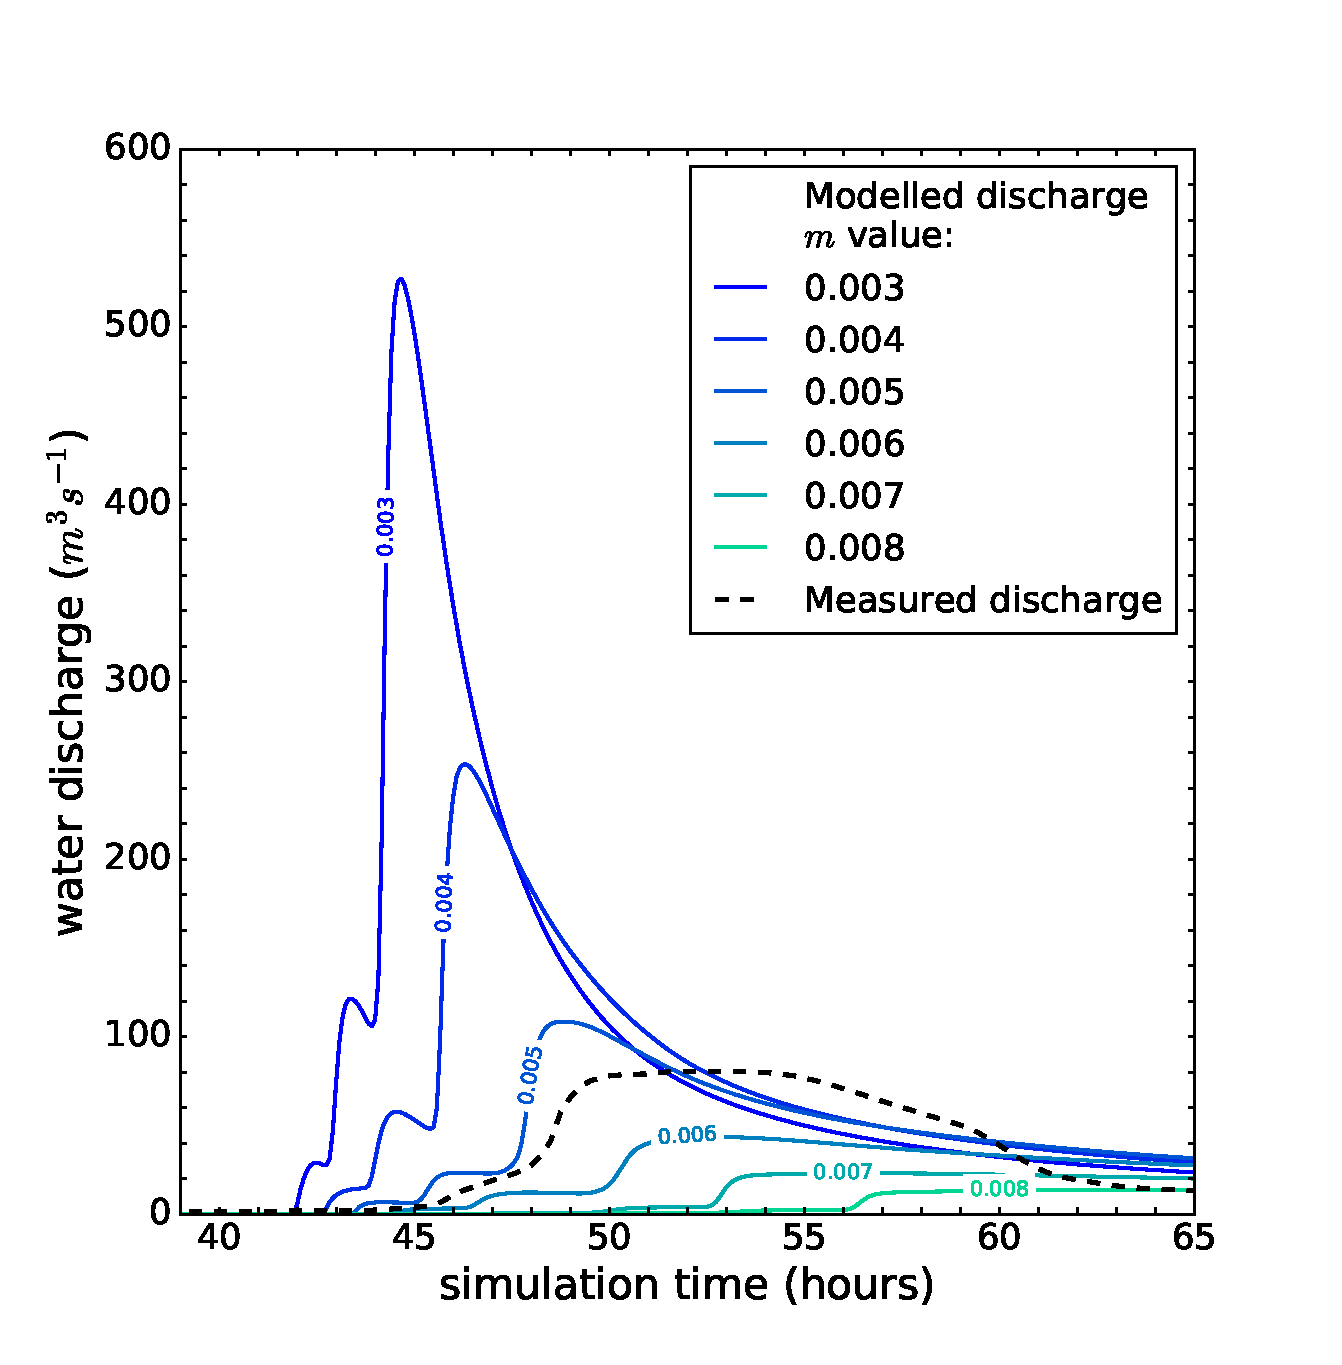
\includegraphics[width=11cm]{chp06_figures_scripts/figure_ryedale_M_sens.eps}
\caption{Discharge at Ryedale catchment outlet for varying values of the TOPMODEL \(m\) parameter. The measured discharge at the catchment gauging station is overlain in dashed line. The results from the simulations with \(m\) \textgreater \ 0.008 are omitted for clarity due to the low peak discharges they produced.}
\label{fig_topmodel_m_ryedale}
\end{figure}

\subsection{Catchment hydrology}

%Comparisons with the actual hydrographs from the gauged basins?

At the catchment scale, hydrological response was sensitive to both the rainfall resolution and the choice of erosional model. For all catchments, higher resolution rainfall input data resulted in a flashier storm hydrograph, with catchments reaching their peak discharge sooner than the uniform rainfall cases. Maximum river discharges were also higher when using higher resolution rainfall data. The choice of erosion model also influenced the hydrograph response. When catchment erosion was modelled using a transport-limited case, peak discharges were higher, but the timing of hydrograph peaks remained very similar for each case. The difference in peak discharges were minimal when comparing the detachment-limited cases to the hydrological-only models.

\subsection{Catchment sediment flux}
% General description of all results.
Sediment flux followed a similar pattern to that observed in water discharge from the catchment. For all catchments and events simulated, sediment flux from the catchment was higher in the simulations using higher resolution rainfall input data. The patterns of peak sediment discharge also mirrored that of water discharge, with sediment flux peaking earlier in the simulations with higher resolution rainfall inputs. 

\subsection{Local variations in catchment erosion}

% Plan view erosion diff maps

\section{Discussion}

\subsection{Implications for longer-term landscape evolution}
\textit{Some discussion on how these results scale-up to longer term landscape evolution. I.e. How many storms of similar magnitude would be needed to reach longer term erosion rates? Does this correspond to known longer term erosion rates of similar upland landscapes?}

%%%%%%%%%%%%%%%%%%%%%
\section{Conclusions}  %% \conclusions[modified heading if necessary]
%%%%%%%%%%%%%%%%%%%%%
Text.



\section{Fixed parameters}

\textit{A table showing the other parameters used in the simulations (All of which remain fixed for each simulation)}

The following table lists the parameters that were held constant for all simulations.
